\documentclass{standalone}
\usepackage{mintikz}

\begin{document}
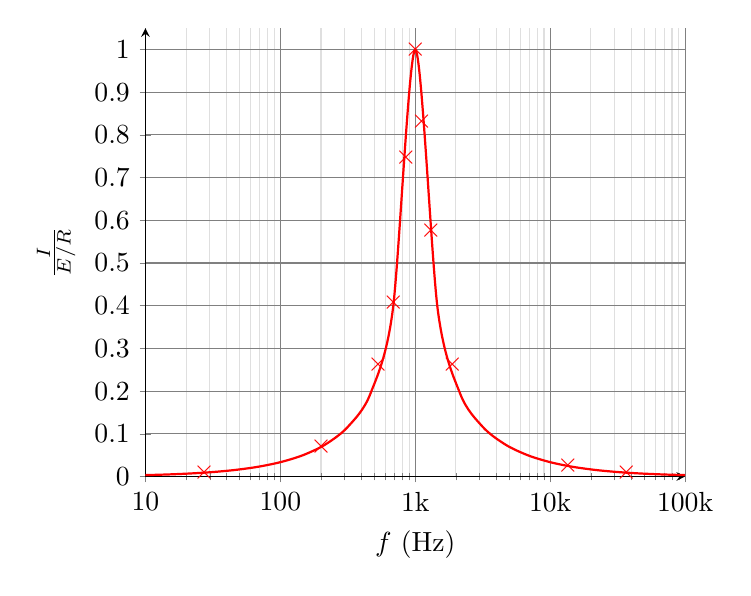
\begin{tikzpicture}[]
    \begin{semilogxaxis}[
        xmin=1e-2, xmax=1e2,
        ymin=0, ymax=1.05,
        xlabel={$f$ (Hz)}, ylabel=$\DS\frac{I}{E/R}$,
        xtick={1e-2, 1e-1, 1e0, 1e1, 1e2},
        xticklabels={10, 100, 1k, 10k, 100k},
        ytick={0, 0.1, ..., 1.1},
        axis lines=left,
        grid=both,
        major grid style={black!50},
        minor grid style={gray!25},
        clip=false]
        \def\Q{3}
        \addplot[
        domain=1e-2:1e2,
        smooth, thick, red]
        {1/sqrt(1+\Q^2*(\x-1/\x)^2)}
        node[pos=0.1] {$\times$}
        node[pos=0.3] {$\times$}
        node[pos=0.4] {$\times$}
        node[pos=0.43] {$\times$}
        node[pos=0.47] {$\times$}
        node[pos=0.5] {$\times$}
        node[pos=0.52] {$\times$}
        node[pos=0.55] {$\times$}
        node[pos=0.6] {$\times$}
        node[pos=0.8] {$\times$}
        node[pos=0.9] {$\times$}
        ;
        % \draw[dashed, thick]
        % (axis cs:1e-2,-3) -|
        % (axis cs:1e0,-30);
    \end{semilogxaxis}
\end{tikzpicture}
\end{document}
